% TODO
% confirm max. points lost method


\documentclass[11pt,
			   %10pt, 
               %hyperref={colorlinks},
               aspectratio=169,
               hyperref={colorlinks}
               ]{beamer}
\usetheme{Singapore}
\usecolortheme[snowy, cautious]{owl}

\usepackage[utf8]{inputenc}
\usepackage[T1]{fontenc}
\usepackage[american]{babel}
\usepackage{graphicx}
\usepackage{hyperref}

\hypersetup{
    colorlinks=true,
    urlcolor=[rgb]{1,0,1},
    linkcolor=[rgb]{1,0,1}}
\definecolor{magenta}{RGB}{255, 0, 255}

\usepackage[natbib=true,style=numeric,backend=bibtex,useprefix=true]{biblatex}

\definecolor{OwlGreen}{RGB}{75,0,130} % easier to see
\setbeamertemplate{bibliography item}{\insertbiblabel}
\setbeamerfont{caption}{size=\footnotesize}
\setbeamertemplate{frametitle continuation}{}

\setcounter{tocdepth}{1}
\renewcommand*{\bibfont}{\scriptsize}
\addbibresource{bibliography.bib}

\renewcommand*{\thefootnote}{\fnsymbol{footnote}}

\usenavigationsymbolstemplate{}
\setbeamertemplate{footline}{%
    \raisebox{5pt}{\makebox{\hfill\makebox[20pt]{\color{gray}
          \scriptsize\insertframenumber}}}\hspace*{5pt}}

\usepackage{epigraph}
% \epigraphsize{\small}% Default
\setlength\epigraphwidth{14cm}
\setlength\epigraphrule{0pt}
\usepackage{etoolbox}
\makeatletter
\patchcmd{\epigraph}{\@epitext{#1}}{\itshape\@epitext{#1}}{}{}
\makeatother

\author{Patrick Hall}
%\thanks{\tiny{This material is shared under a \href{https://creativecommons.org/licenses/by/4.0/deed.ast}{CC By 4.0 license} which allows for editing and redistribution, even for commercial purposes. However, any derivative work should attribute the author and H2O.ai.}}
\title{Responsible Machine Learning: A Primer}
\logo{
\includegraphics[height=8pt]{img/h2o_logo.png}}
\institute{\href{https://www.h2o.ai}{H\textsubscript{2}O.ai}}
\date{\today}
\subject{}

\begin{document}
	
	\maketitle
	
	\begin{frame}
	
		\frametitle{Contents}
		
		\tableofcontents{}
		
	\end{frame}

\renewcommand*{\thefootnote}{\arabic{footnote}}

%-------------------------------------------------------------------------------
	\section{Time to Grow Up}
%-------------------------------------------------------------------------------

	%\subsection*{} % just for progress indicator

	\begin{frame}[t]
		
		\frametitle{Time to Grow Up}
		
		\centering

		Machine learning (ML) is about 60 years old.
		\vspace{10pt}
		
		\begin{columns}
				
			\column{0.5\linewidth}
			\centering
			\tiny{Image: \href{https://webdocs.cs.ualberta.ca/~chinook/project/legacy.html}{University of Alberta}}\\
			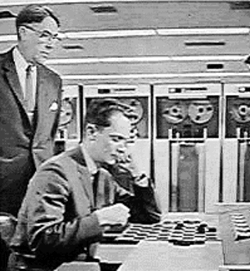
\includegraphics[height=120pt]{img/samuel_sm.jpeg}\\	
			% image: https://webdocs.cs.ualberta.ca/~chinook/project/legacy.html
			\normalsize{Then.}			
				
			\column{0.5\linewidth}
			\centering
			\tiny{Image: \href{https://www.bloomberg.com/news/articles/2014-08-07/silicon-valley-tech-entrepreneurs-behind-the-stereotype}{Bloomberg}}\\
			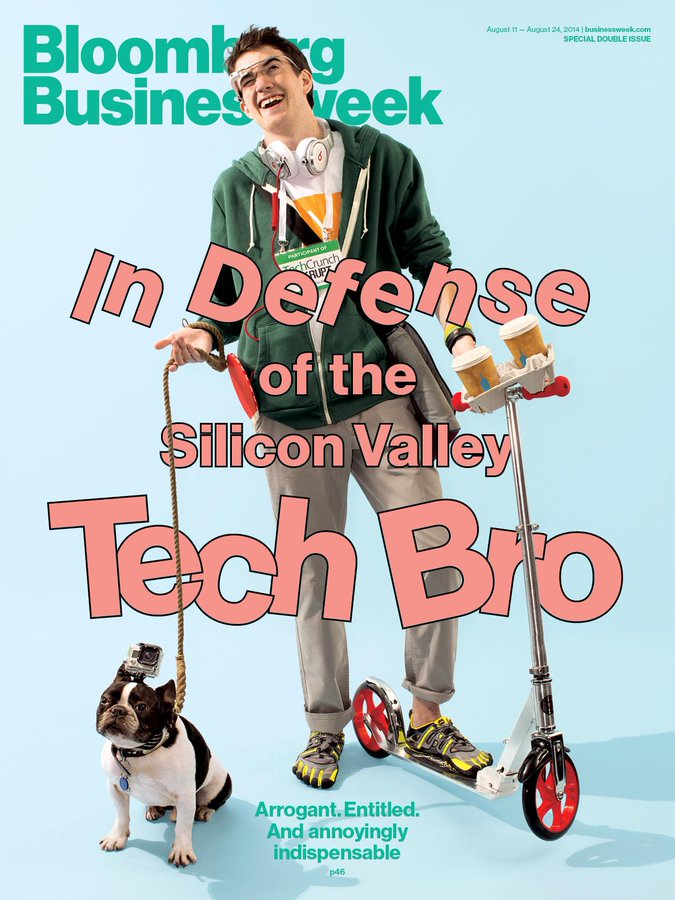
\includegraphics[height=130pt]{img/bi_tech_bro.jpeg}\\
			\normalsize{Now.}
		
		\end{columns}
		
		(So why don't we act like it?)
		
		% Benjamin button
		% Maybe all of society is just decaying		
		
	\end{frame}
	
	
%-------------------------------------------------------------------------------
	\section{Risky Business?}
%-------------------------------------------------------------------------------

	\subsection*{} % just for progress indicator

	\begin{frame}[t]
		
		\frametitle{Risky Business?}		
		\centering
		All technologies present risks. ML is no different.\\
		\vspace{10pt}
		\tiny{Image: \href{https://en.wikipedia.org/wiki/Boeing_707}{Wikipedia}}\\		
		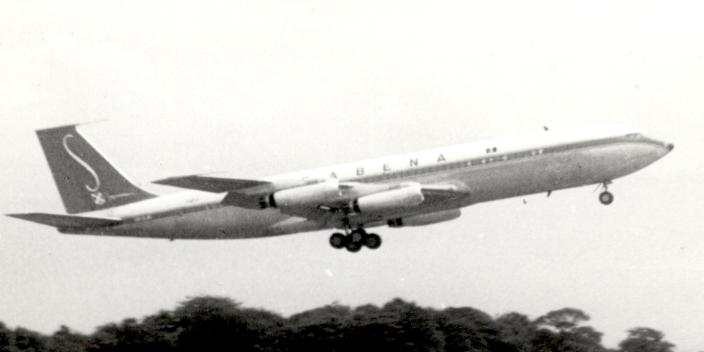
\includegraphics[height=90pt]{img/707.jpg}\\
		\vspace{10pt}
		\normalsize{About 60 years into aviation technology, the Boeing 707 was born. This model of plane has been involved in 261 accidents, causing a total of 3,039 fatalities, over it's long deployment. It was still flying \textit{and crashing} in 2019.}
		% image and info: https://en.wikipedia.org/wiki/Boeing_707
		% do you think ML models are as carefully crafted and tested as this airplane?
		
	\end{frame}
	
	\subsection*{} % just for progress indicator

	\begin{frame}
		
		\frametitle{But What Could Go Wrong??!}
		
		\begin{columns}		
		
			\column{0.5\linewidth}
		
			\begin{itemize}
				\item Being wrong.
				\item Discrimination.
				\item ``Computer Says No.''
				\item Privacy harms.
				\item Security vulnerabilities.
				\item Reputational damage.
				\item Noncompliance.
				\item Fines and financial losses.
				\item Systemic failures.
			\end{itemize}
		
			% headline pic instead
			\column{0.5\linewidth}
			\begin{center}
			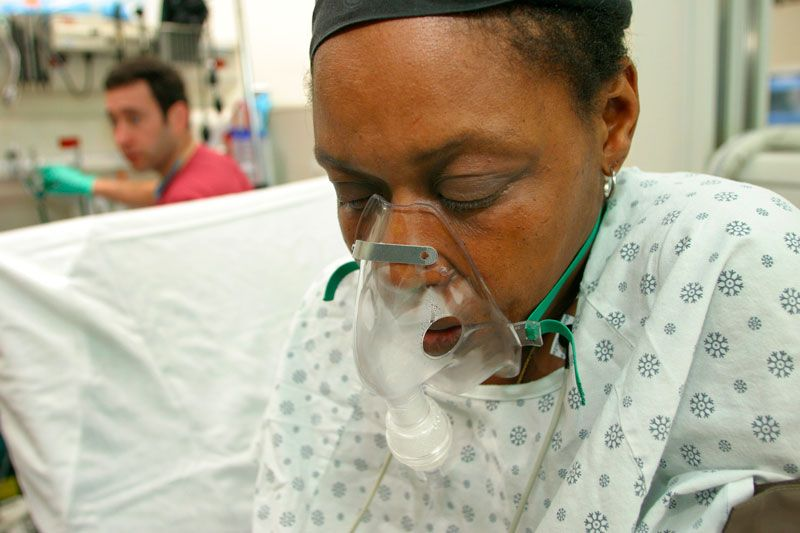
\includegraphics[height=100pt]{img/nature.jpg}
			\end{center}
			\vspace{10pt}
			“Millions of black people affected by racial bias in health-care algorithms”\\ --- \href{https://www.nature.com/articles/d41586-019-03228-6}{Nature}, 24 Oct. 2019

		\end{columns}	
		% also: 
		% facial recognition in hong kong
		% COMPAS
		% target privacy violation
		% tai being poisoned to become discriminatory
		% apple/goldman sachs
		% amazon hiring 
		% gendershades		
				
	\end{frame}
	
	% go fast and break people's lives

%-------------------------------------------------------------------------------
	\section{Vocabulary Quiz}
%-------------------------------------------------------------------------------

	%\subsection*{} % just for progress indicator

	\begin{frame}
		
		\frametitle{Vocabulary Quiz}
		
		\begin{itemize}
			\item \textbf{Explainable AI} (XAI): the ability to analyze a ML model after it has been developed. 
			\item \textbf{Interpretable ML}: transparent model architectures and increasing how intuitive and understandable ML models can be.
			\item \textbf{Ethical AI}: sociological fairness in ML model predictions (i.e., whether one category of person is being weighted unequally). 
			\item \textbf{AI Security}: debugging and deploying ML models with similar counter-measures against insider and cyber threats as would be seen in traditional software.
			\item \textbf{Human-centered AI}: user interactions with AI and ML systems.		
		\end{itemize}
		
	\end{frame}


%-------------------------------------------------------------------------------
	\section{Responsible ML}
%-------------------------------------------------------------------------------

	%\subsection*{} % just for progress indicator

	\begin{frame}
	
	\frametitle{Responsible ML}
		
		\begin{columns}
				
			\column{0.5\linewidth}
			\centering
			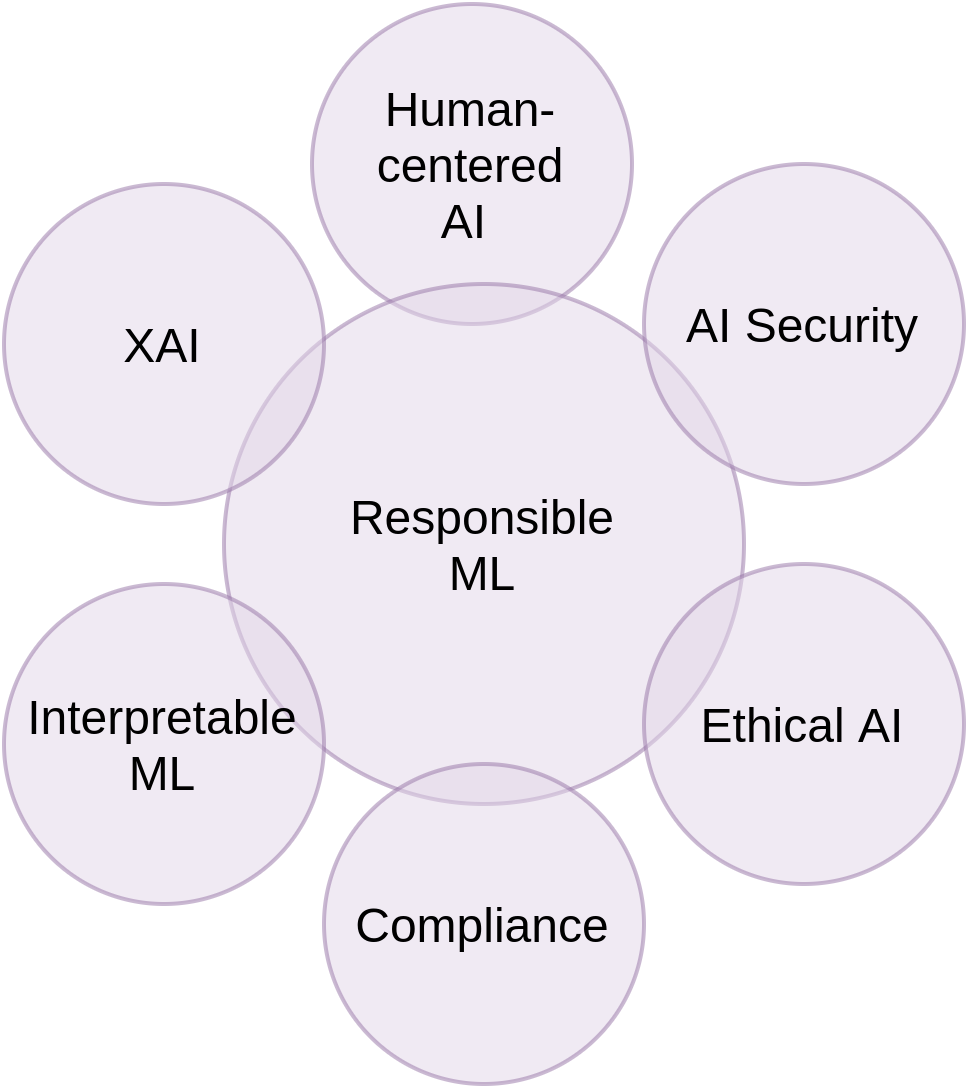
\includegraphics[height=170pt]{img/responsible_ml.png}
			
			\column{0.5\linewidth}
			\noindent Responsible ML is essentially a combination of existing technologies and best practices that a \textit{responsible} organization would employ to mitigate ML risks, including regulatory compliance processes.
			
			\end{columns}
		
	\end{frame}

%-------------------------------------------------------------------------------
	\section{I Fought the Law ...}
%-------------------------------------------------------------------------------

	%\subsection*{} % just for progress indicator

	\begin{frame}[t]
		
		\frametitle{I Fought the Law ...}
			
		\begin{columns}			
			
			\column{0.5\linewidth}
					\noindent AI and law are colliding.\\
					\vspace{5pt}
			\noindent Government agencies in \textit{at least} ...
			\begin{itemize}\small
				\item \href{https://bit.ly/2tRJwmy}{Canada}
				\item \href{https://bit.ly/2UKSAVh}{Germany}
				\item \href{https://bit.ly/39xWLIu}{Netherlands}
				\item \href{https://www.pdpc.gov.sg/Resources/Model-AI-Gov}{Singapore}
				\item \href{https://bit.ly/38ovaJh}{UK}
				\item \href{https://bit.ly/2wcJOW1}{USA}
			\end{itemize}\normalsize
			\vspace{5pt}
			... have issued or proposed AI-specific guidance.			
		
			\column{0.5\linewidth}
			\begin{center}
			
\includegraphics[height=110pt]{img/syri.png}
			\end{center}
			\small
			“Government’s fraud algorithm SyRI breaks human rights, privacy law” --- \href{https://www.dutchnews.nl/news/2020/02/governments-fraud-algorithm-syri-breaks-human-rights-privacy-law/}{dutchnews.nl}, Feb. 5 2020
			
		\end{columns}\normalsize
		
	\end{frame}
	
	% Are you planning on doing AI in one of these countries?

%-------------------------------------------------------------------------------
	\section{Transparency Paradox}
%-------------------------------------------------------------------------------

	%\subsection*{} % just for progress indicator

	\begin{frame}[t]
		
		\frametitle{Transparency Paradox}
		
		\epigraph{``[T]here are two ways of constructing a software design: One way is to make it so simple that there are \textit{obviously} no deficiencies and the other way is to make it so complicated that there are no \textit{obvious} deficiencies.''}{--- C.A.R. Hoare, \href{http://www.cs.fsu.edu/~engelen/courses/COP4610/hoare.pdf}{1980 ACM Turing Award Lecture}}		
		
		\begin{itemize}
		\item XAI presents \href{https://arxiv.org/abs/1907.00164}{privacy risks}.
		\item Interpretable models, XAI, and the model documentation they enable \href{https://www.hhs.gov/about/news/2018/06/18/judge-rules-in-favor-of-ocr-and-requires-texas-cancer-center-to-pay-4.3-million-in-penalties-for-hipaa-violations.html}{can increase legal liability} if they show an organization was aware of a serious problem.
		\item Consider conducting mission-critical ML projects and risk assessments\\ \href{https://hbr.org/2019/12/the-ai-transparency-paradox}{under legal privilege}.
		\end{itemize}
		
		
	\end{frame}


%-------------------------------------------------------------------------------
	\section{References}
%-------------------------------------------------------------------------------

	\begin{frame}
	
		\frametitle{References}	
		
		\normalsize{Awesome machine learning interpretability metalist}\\
		\scriptsize{\url{https://github.com/jphall663/awesome-machine-learning-interpretability}}\\
		\vspace{10pt}
		\normalsize{\textit{An Introduction to Machine Learning Interpretability - 2nd Edition}}\\
		\scriptsize{\url{https://www.h2o.ai/oreilly-mli-booklet-2019}}\\
		\vspace{10pt}
		\normalsize{\textit{Proposed Guidelines for the Responsible Use of Explainable Machine Learning}}\\
		\scriptsize{\url{https://arxiv.org/pdf/1906.03533.pdf}}
								
	
		
	\end{frame}

\end{document}